
\section{Scénario}

Les joueurs devront se connecter sur un serveur afin d'accéder à la partie. Le serveur hébergera la partie en traitant les mécanismes de la partie en arrière-plan. Les utilisateurs recevront une interface graphique en provenance du serveur et communiqueront avec cette interface pour jouer dans la partie.
Le serveur avertira l'utilisateur lors d'une mauvaise utilisation de l'interface et des requêtes parasites pour le serveur.




La carte s'affiche quand les deux joueurs sont connectés. Ici le joueur 1 peut commencer à jouer.
Nous pouvons voir en haut de la page une barre qui affiche le tour actuel et le nombre total de tour, qui est 38, la phase actuelle et le nombre d'unités restantes.

\begin{figure}[H]
    \centering
    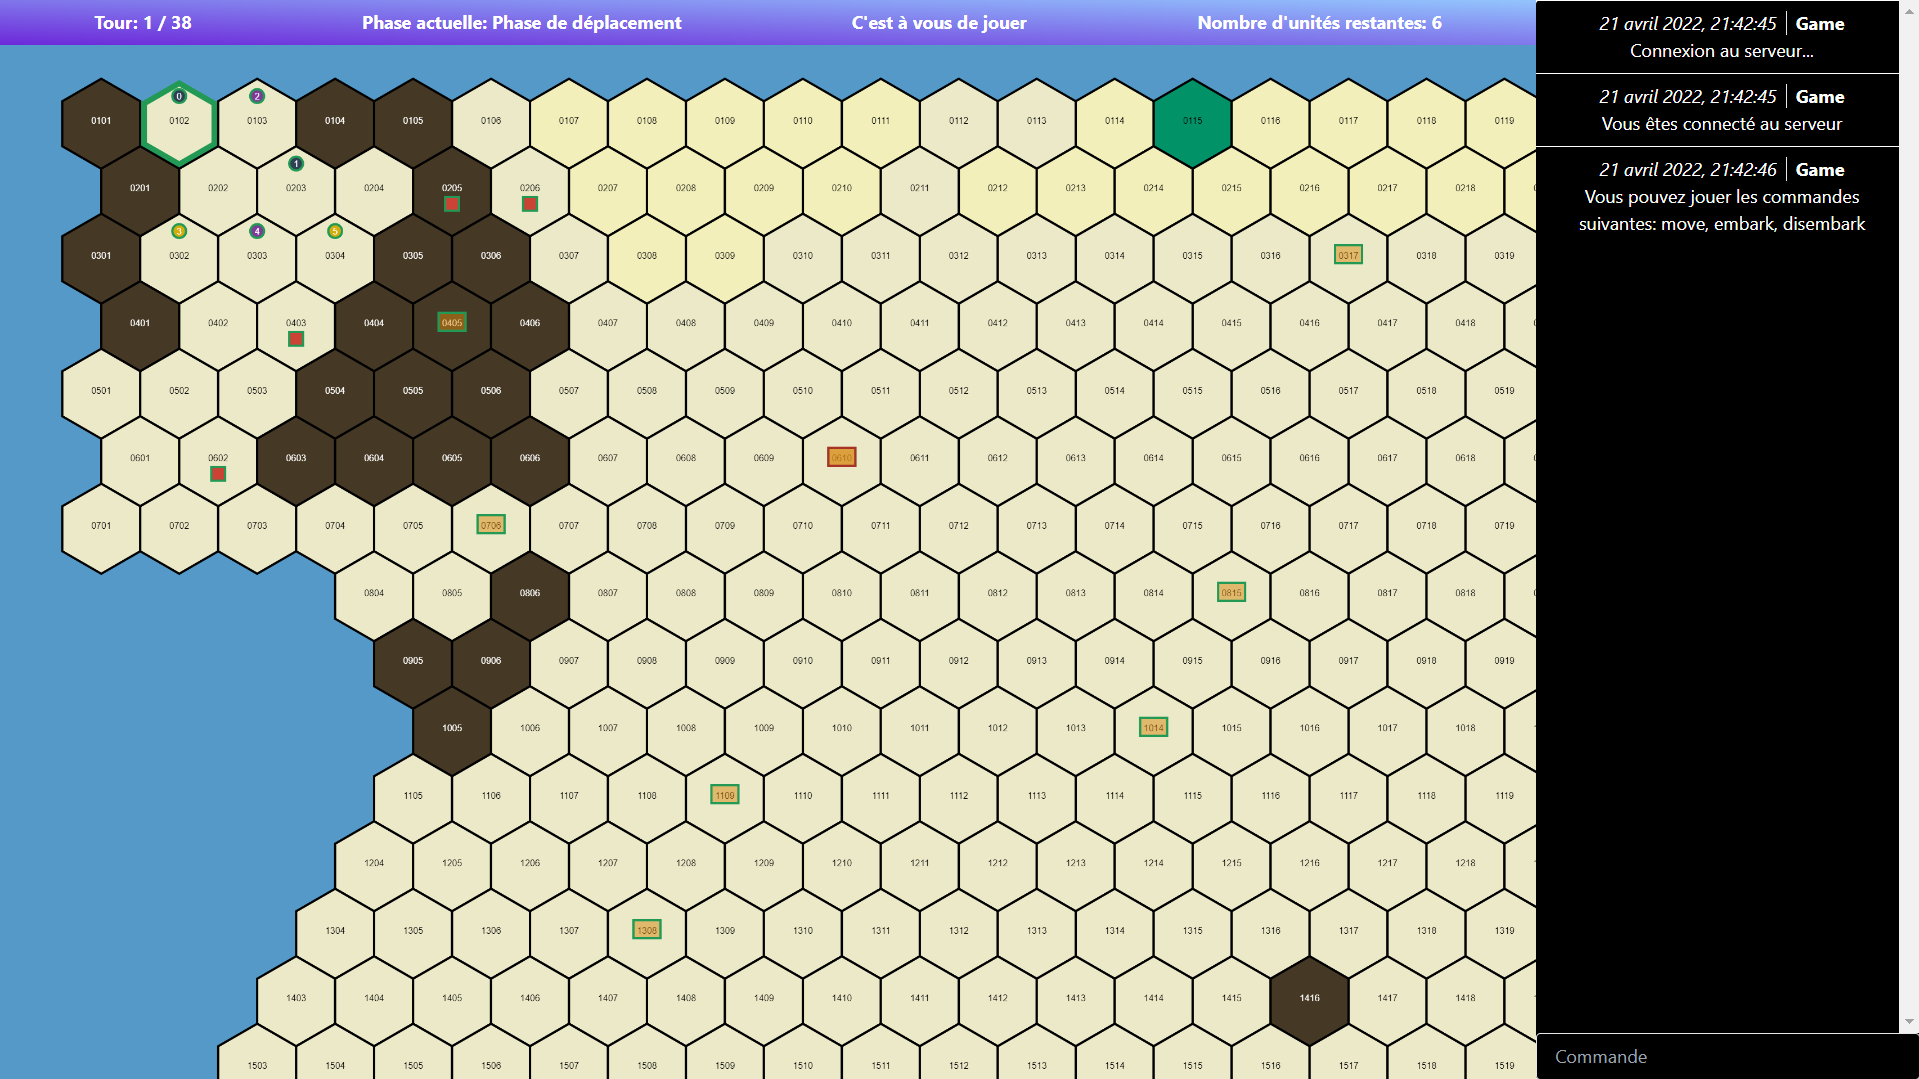
\includegraphics[scale=0.35]{data/plateau_du_jeu.png}
    \caption{Plateau du jeu Desert Fox}.
\end{figure}

En bas à gauche de la carte une légende(figure \ref{fig:map_legend}) explique les types de terrain et les types d'entités.\\

\begin{figure}[H]
    \centering
    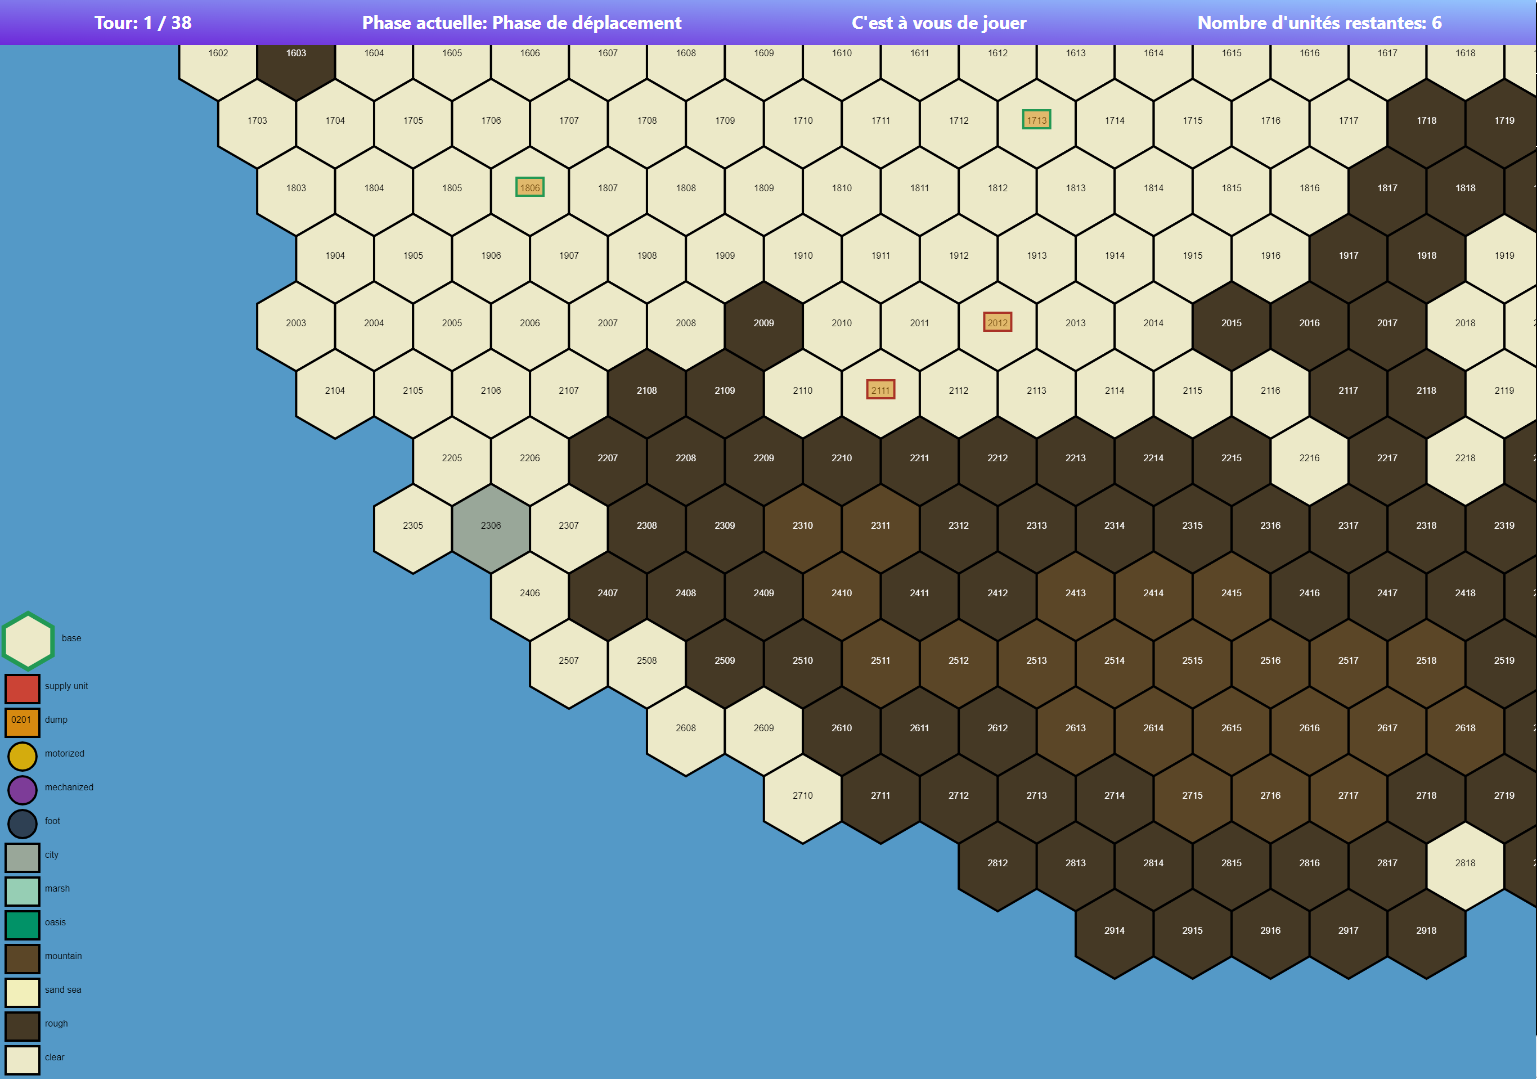
\includegraphics[scale=0.45]{data/Bas_de_map.png}
    \caption{Bas de la carte du jeu}.
\end{figure}

Le joueur peut effectuer la commande {\tt help}  pour afficher toutes les commandes disponibles du jeu. Voir figure \ref{fig:help_command} pour une illustration.\\

Le joueur peut afficher des informations concernant ses unités dans le terminal.
En tapant \og units \fg{}, le joueur à toutes ses unités présentes avec le mouvement point et  les points de vies.
. Vous pouvez voir un exemple d'utilisation dans l'annexe a la figure \ref{fig:units_command}. \\

Le joueur peut aussi afficher les entités, par exemple les unités, les bases, les dumps et les unités de soutien qui sont présents dans un hexagone.
Cela est possible grâce à la commande {\tt hex}, qui prend en paramètre un identifiant d'hexagone. Voir la figure \ref{fig:hex_command} pour un exemple d'utilisation.\\


Voici la page du joueur 1 qui peut jouer.\\
\begin{figure}[H]
    \centering
    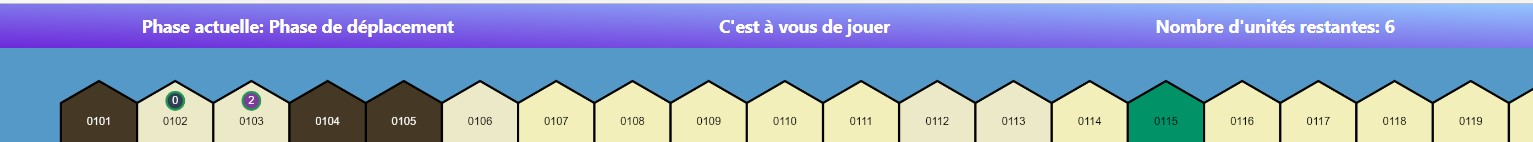
\includegraphics[scale=0.6]{data/player_1_acces.jpg}
    \caption{Barre d'information du joueur 1}.
\end{figure}

Voici la page du joueur 2 qui doit attendre l'adversaire de jouer.\\
\begin{figure}[H]
    \centering
    
\includegraphics[scale=0.6]{data/joueur_2.jpg}
    \caption{Barre d'information du joueur 2}.
\end{figure}

Le joueur qui peut jouer peut faire bouger son unité dans le terminal à droite de l'image.
Nous pouvons voir que l'unité 0 s'est déplacé de l'hexagone \lstinline{0102} à \lstinline{0206}. Le déplacement est valide, car on ne dépasse pas la capacité de mouvement de l'unité (MA).\\

\begin{figure}[H]
    \centering
    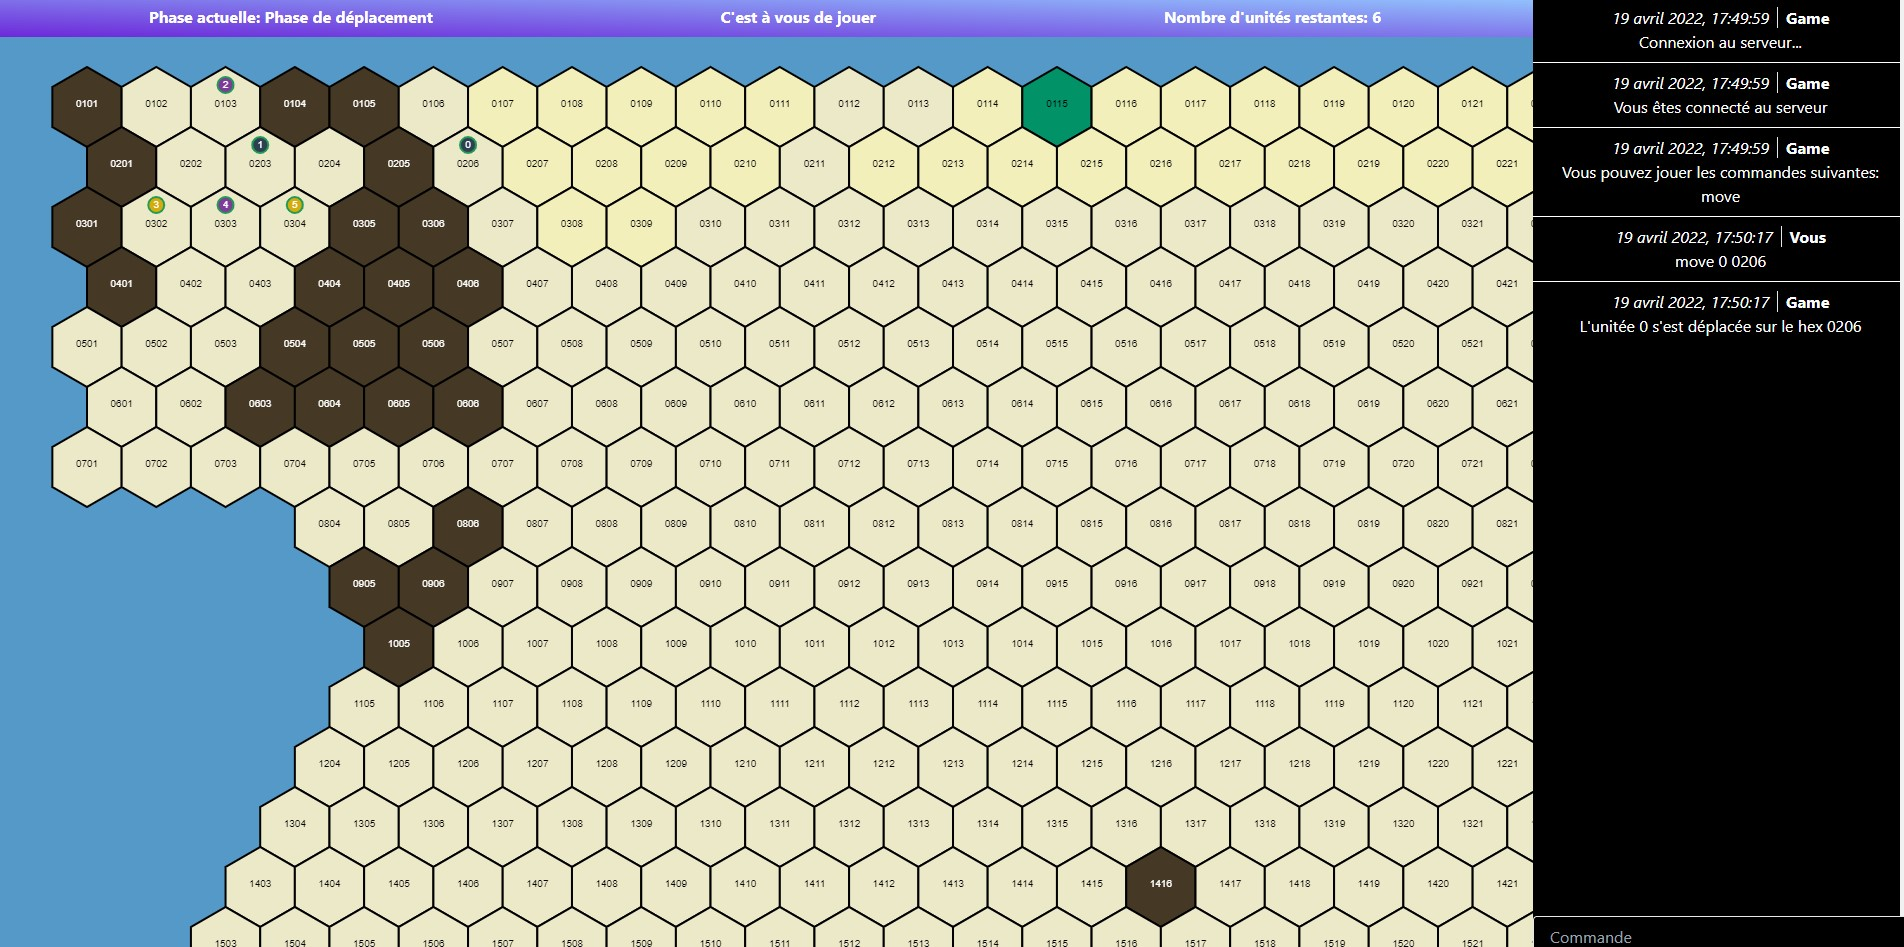
\includegraphics[scale=0.45]{data/move_unit_player_1.jpg}
    \caption{Mouvement de l'unité \lstinline{0} vers l'hexagone \lstinline{0206}}.
\end{figure}

Le joueur peut aussi utiliser une de ses unités de soutien pour bouger soit une unité de type {\tt foot} soit un dump.
Il peut faire cela avec la commande {\tt embark} qui prend en paramètre l'identifiant de l'unité du soutien qui va embarquer, ainsi que l'identifiant de l'unité qui va etre embarquée. Voici un exemple :\\

\begin{figure}[H]
    \centering
    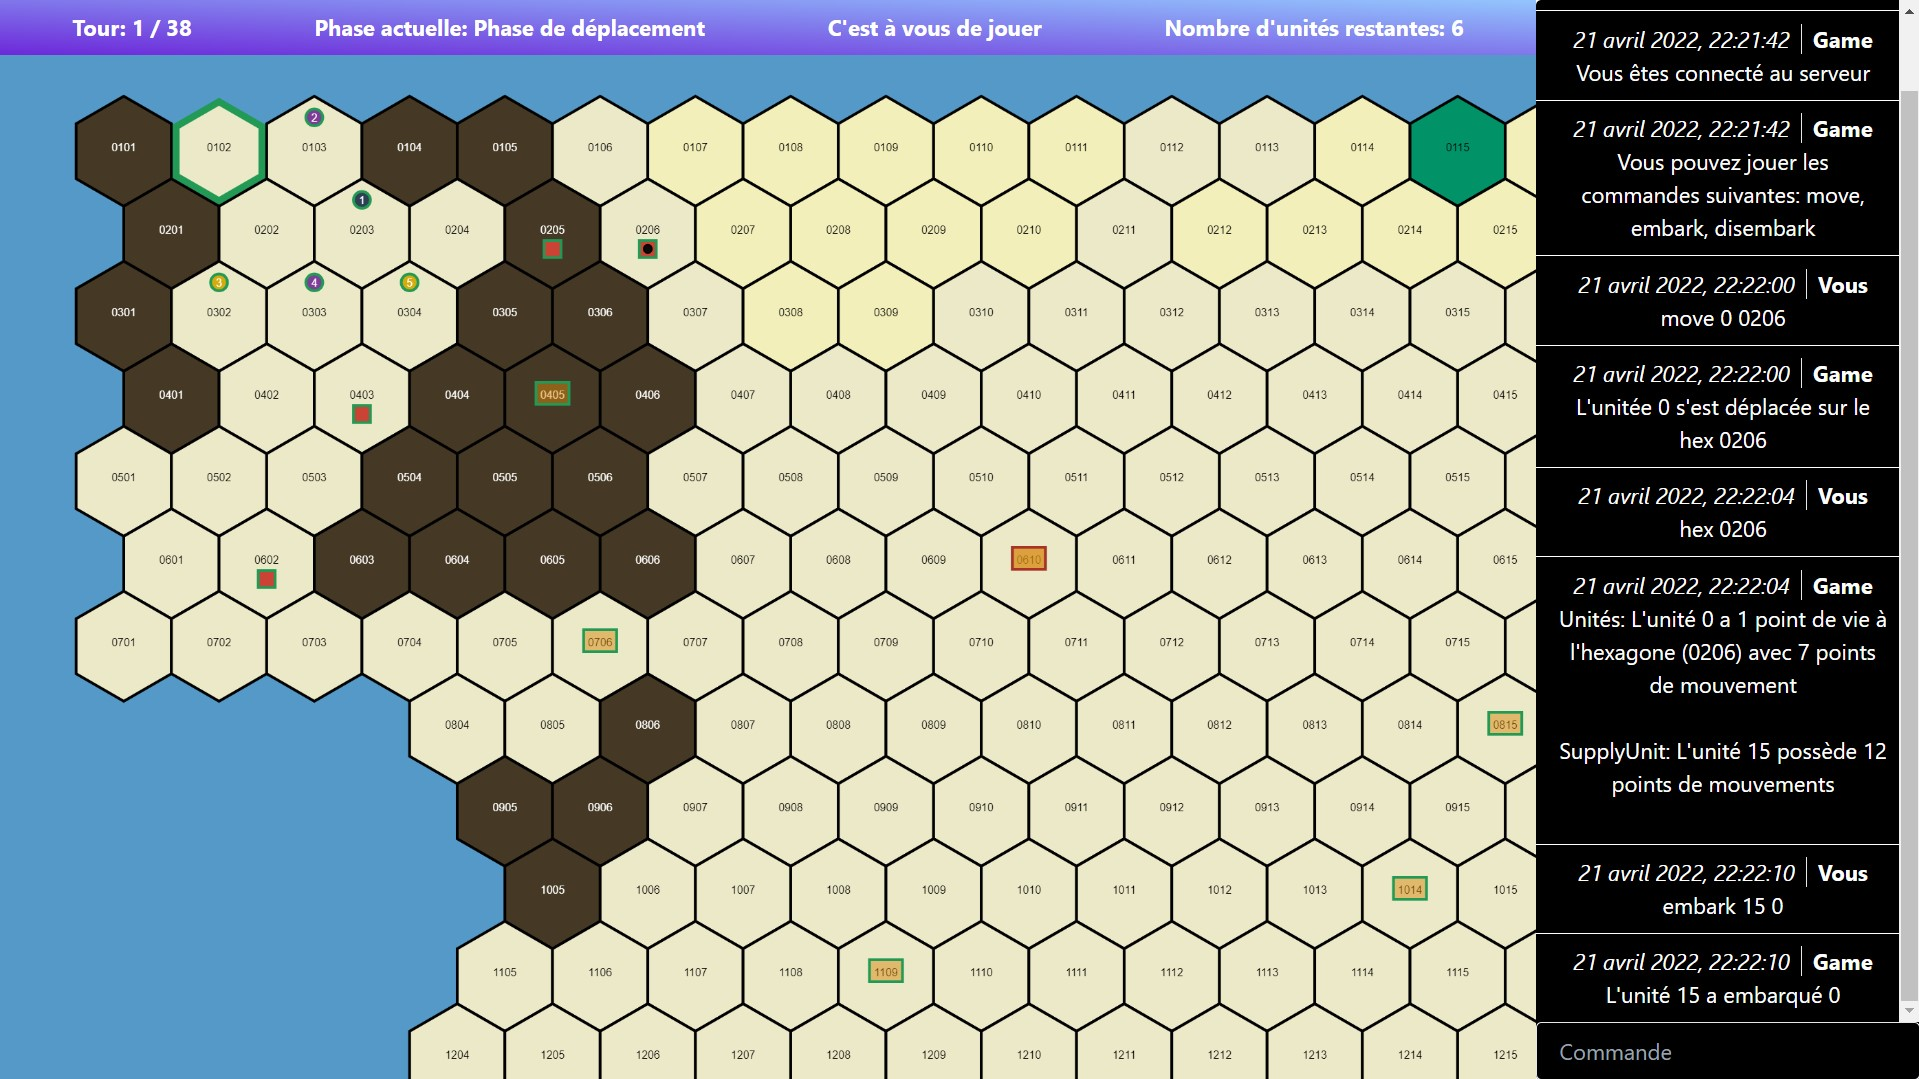
\includegraphics[scale=0.35]{data/Embark_command.jpg}
    \caption{Embarquement de l'unité \lstinline{0} dans l'unité de soutien  \lstinline{15}}.
\end{figure}

Il faut noter que l'unité qui est embarqué est inexistante dans la carte. Elle ne peut donc pas bouger elle meme, ni attaquer. Si l'unité du soutien a embarqué une unité, elle bougera avec elle. Dans la figure ci-dessous nous pouvons voir que si nous embarquons un dump, qui est une entité qui ne peut pas bouger elle meme, nous pouvons la faire bouger avec l'unité de soutien. Ici nous la bougeons de l'hexagone \lstinline{0406} vers l'hexagone \lstinline{0407} \\

\begin{figure}[H]
    \centering
    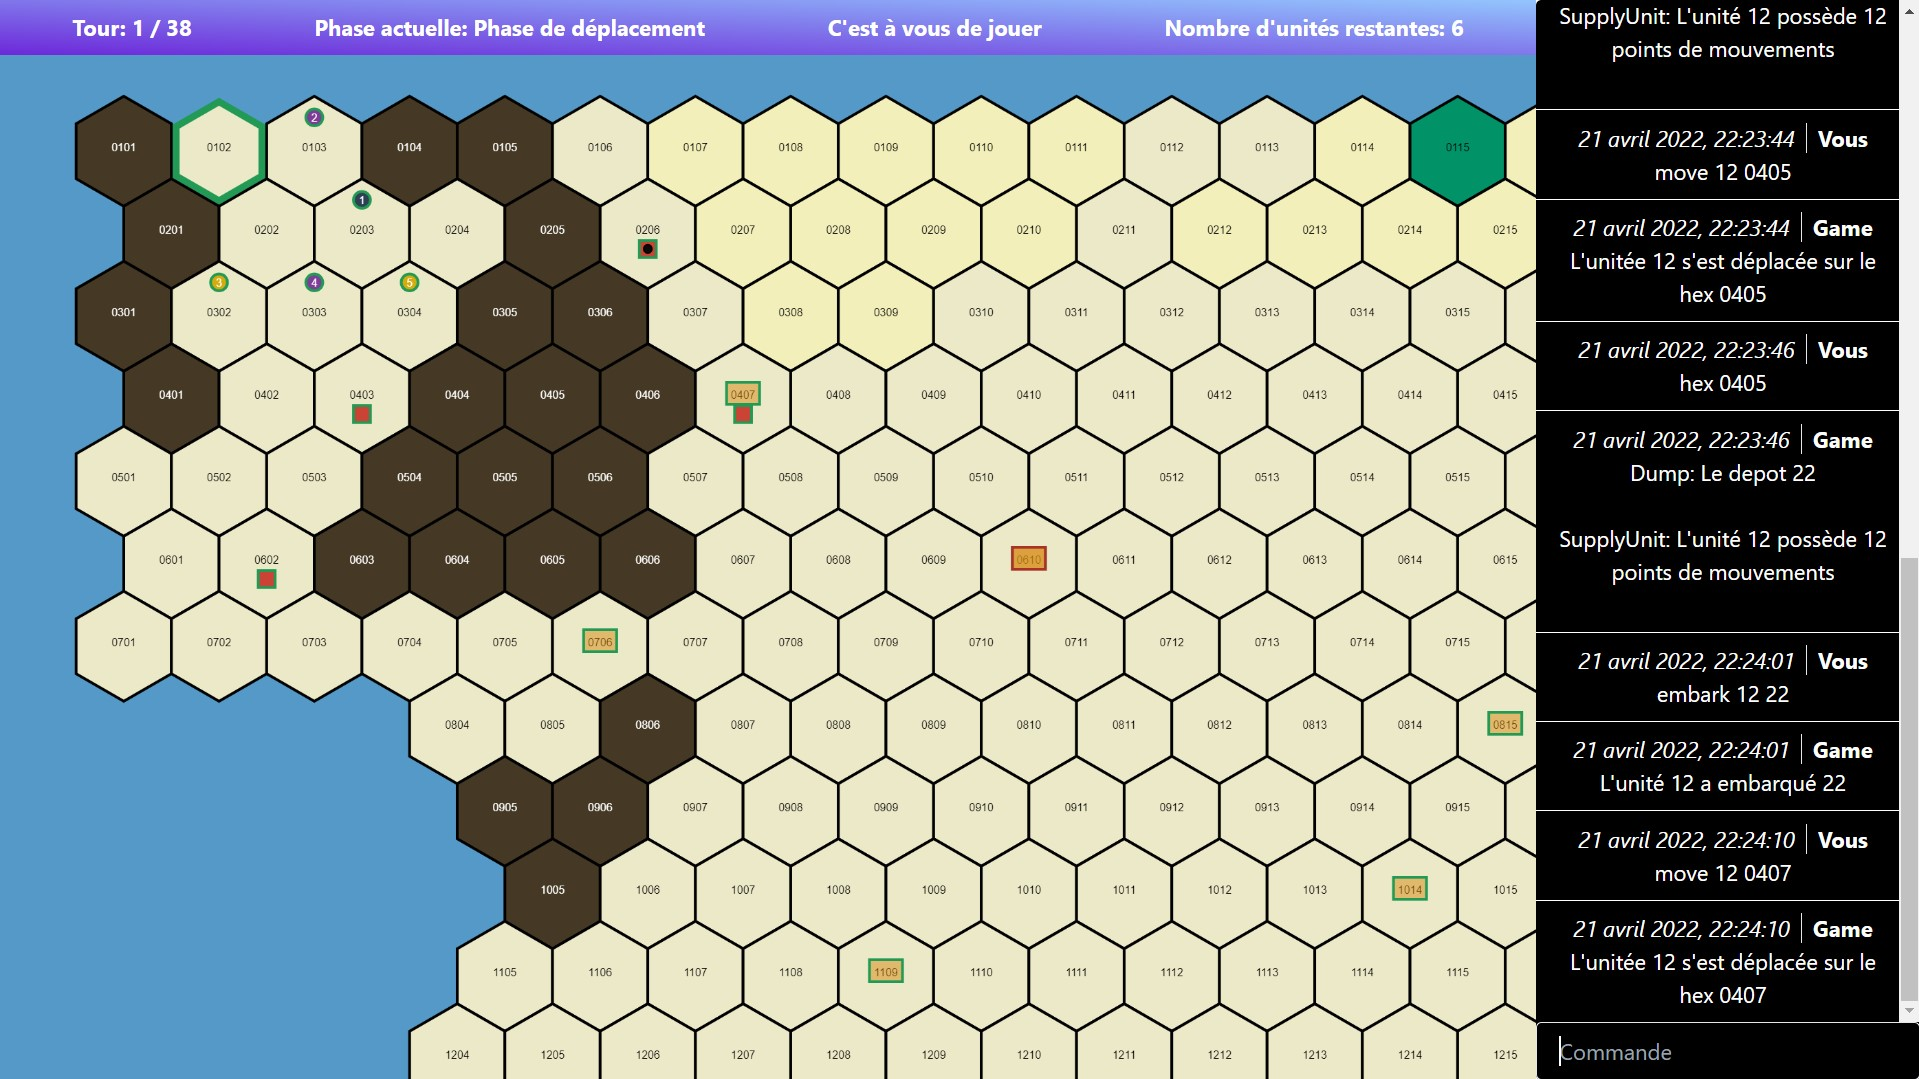
\includegraphics[scale=0.35]{data/Embark_dump.jpg}
    \caption{Embarquement du dump \lstinline{22} dans l'unité de soutien  \lstinline{12} suivi par un déplacement de l'unité du soutien à l'hexagone \lstinline{0407} (avec le dump)}.
\end{figure}

Afin de pouvoir réutiliser l'unité ou l'entité embarquée, nous devons utiliser la commande disembark, laquelle permet de débarquer cette dernière.
Dans la figure ci-dessous nous pouvons voir qu'après avoir bougé l'unité de soutien {\tt 15}, laquelle contient l'unité {\tt 0} et débarquer, l'unité est dorénavant disponible pour un autre mouvement ou action. Elle est aussi affichée à nouveau dans la carte.\\

\begin{figure}[H]
    \centering
    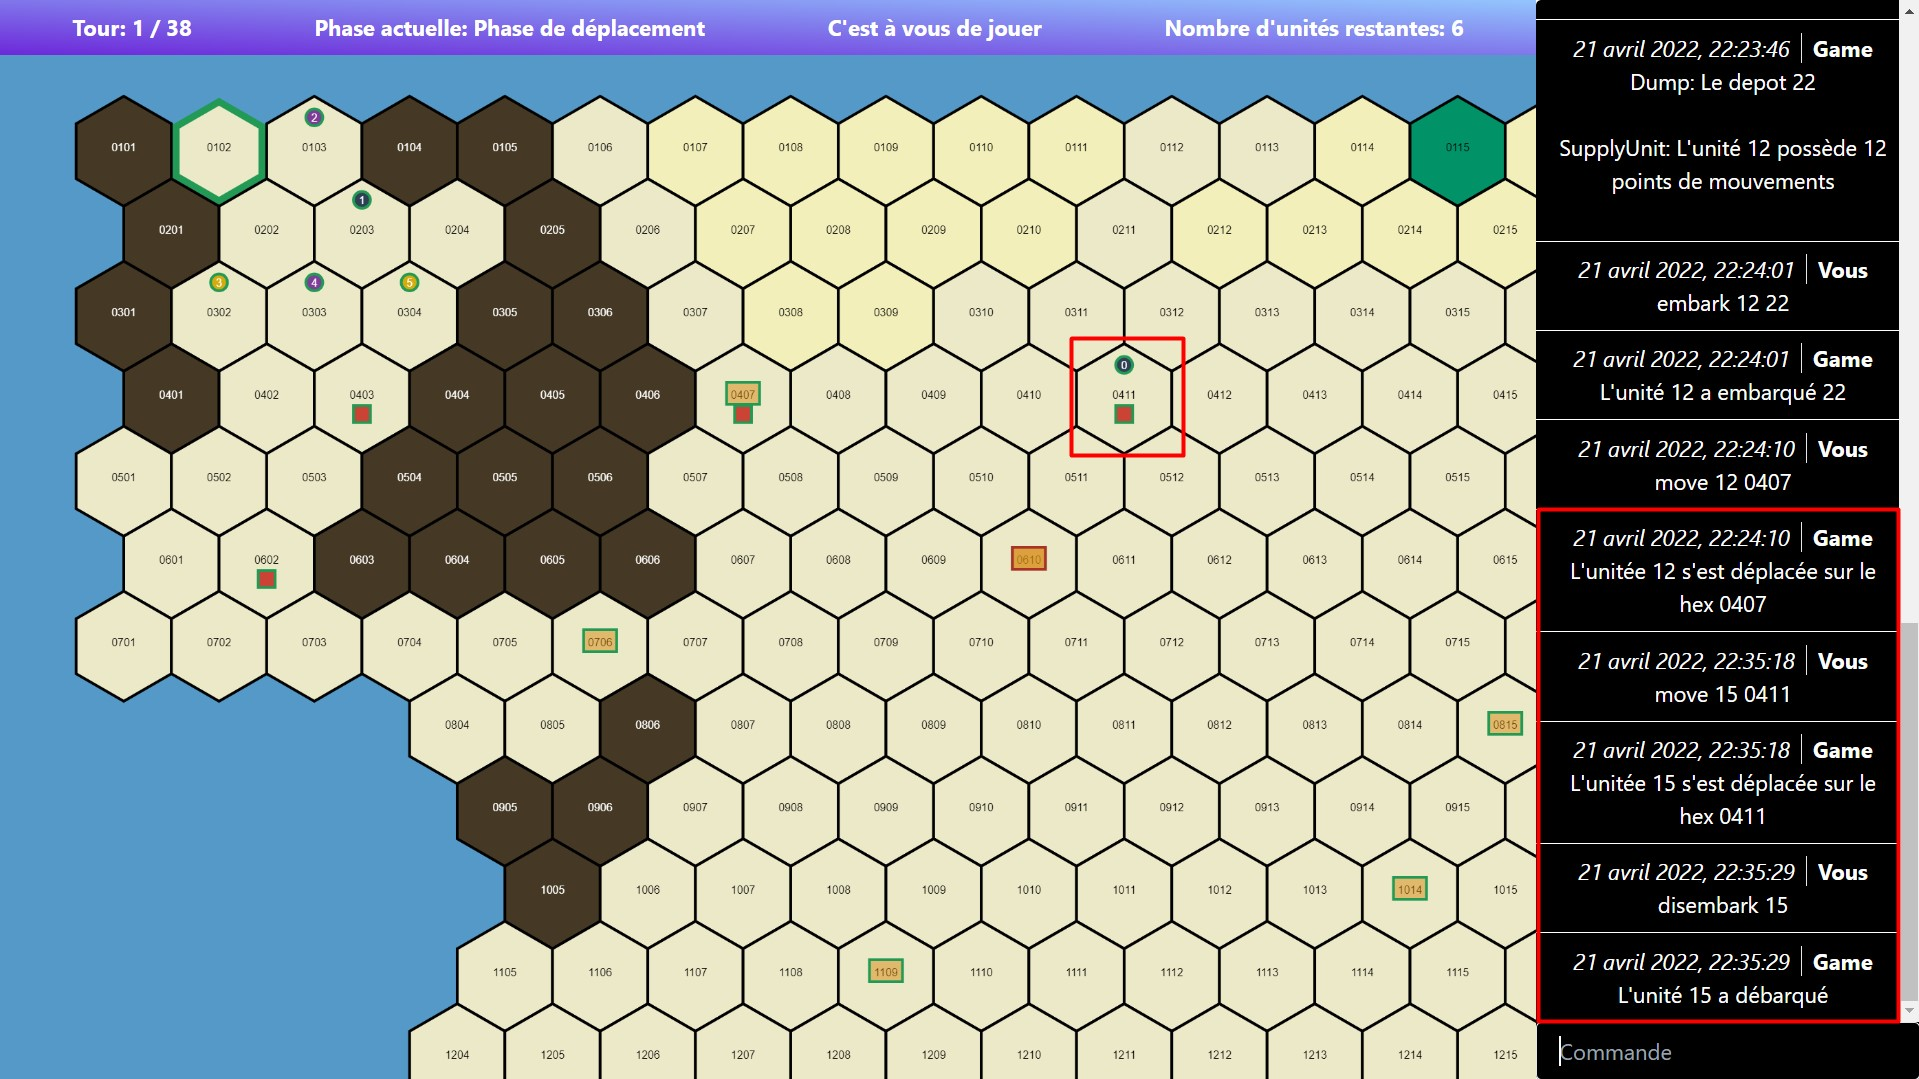
\includegraphics[scale=0.35]{data/Disembark.jpg}
    \caption{Mouvement de l'unité du soutien \lstinline{15}, laquelle contient l'unité \lstinline{0} à l'hexagone \lstinline{0411}, suivi du débarquement de l'unité embarquée}.
\end{figure}

L'utilisateur peut aussi utiliser la commande {\tt attack} pour attaquer une unité adverse. Il faut noter que l'attaque est uniquement possible si l'unité est dans une case adjacente de l'unité adverse. Dans la figure ci-dessous, nous pouvons voir que le deuxième joueur a décidé de se préparer pour une attaque en bougeant son unité {\tt 11} à l'hexagone adjacente de l'unité {\tt 5} de son adversaire.\\

\begin{figure}[H]
    \centering
    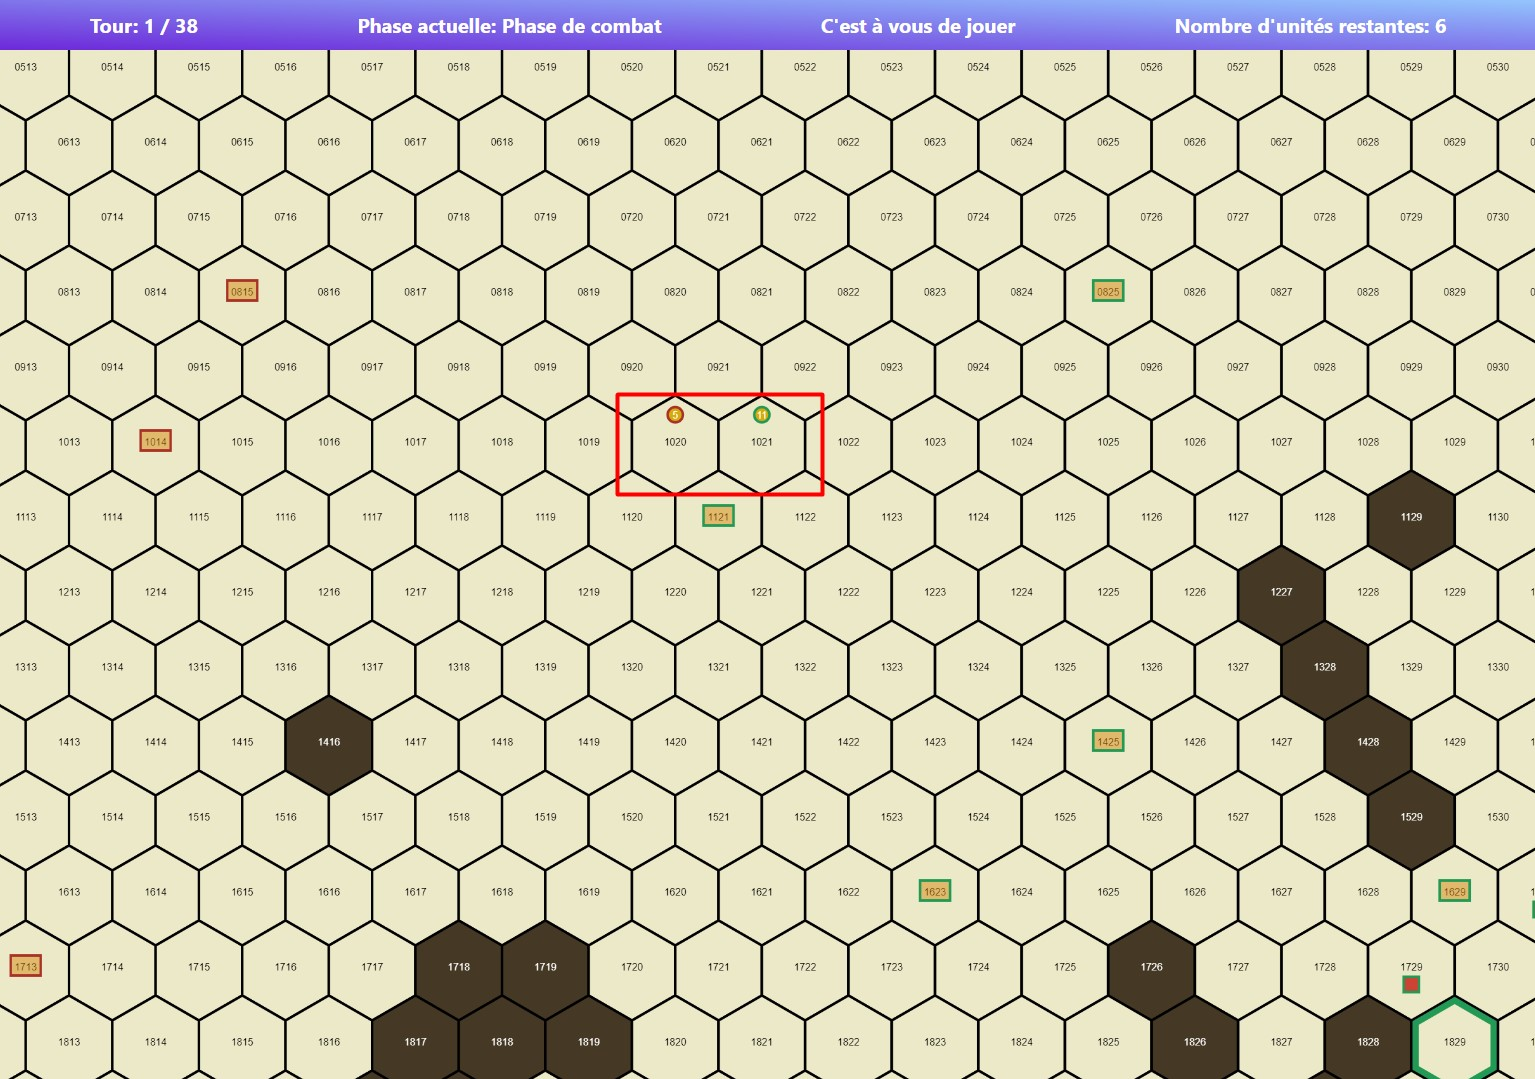
\includegraphics[scale=0.35]{data/beforeAttack.jpg}
    \caption{Mouvement de l'unité \lstinline{11} à l'hexagone \lstinline{1021}, l'hexagone adjacent à \lstinline{1020}, qui contient l'unité \lstinline{5} de l'adversaire }.
\end{figure}

Ensuite, le deuxième joueur lance l'attaque en utilisant la commande {\tt attack} suivie des deux identifiants d'hexagones ( {\tt 1021} {\tt 1020}, respectivement celle de l'attaquant et l'attaqué ). Le résultat du combat est alors affiché dans le terminal pour les deux joueurs : \\

\begin{figure}[H]
    \centering
    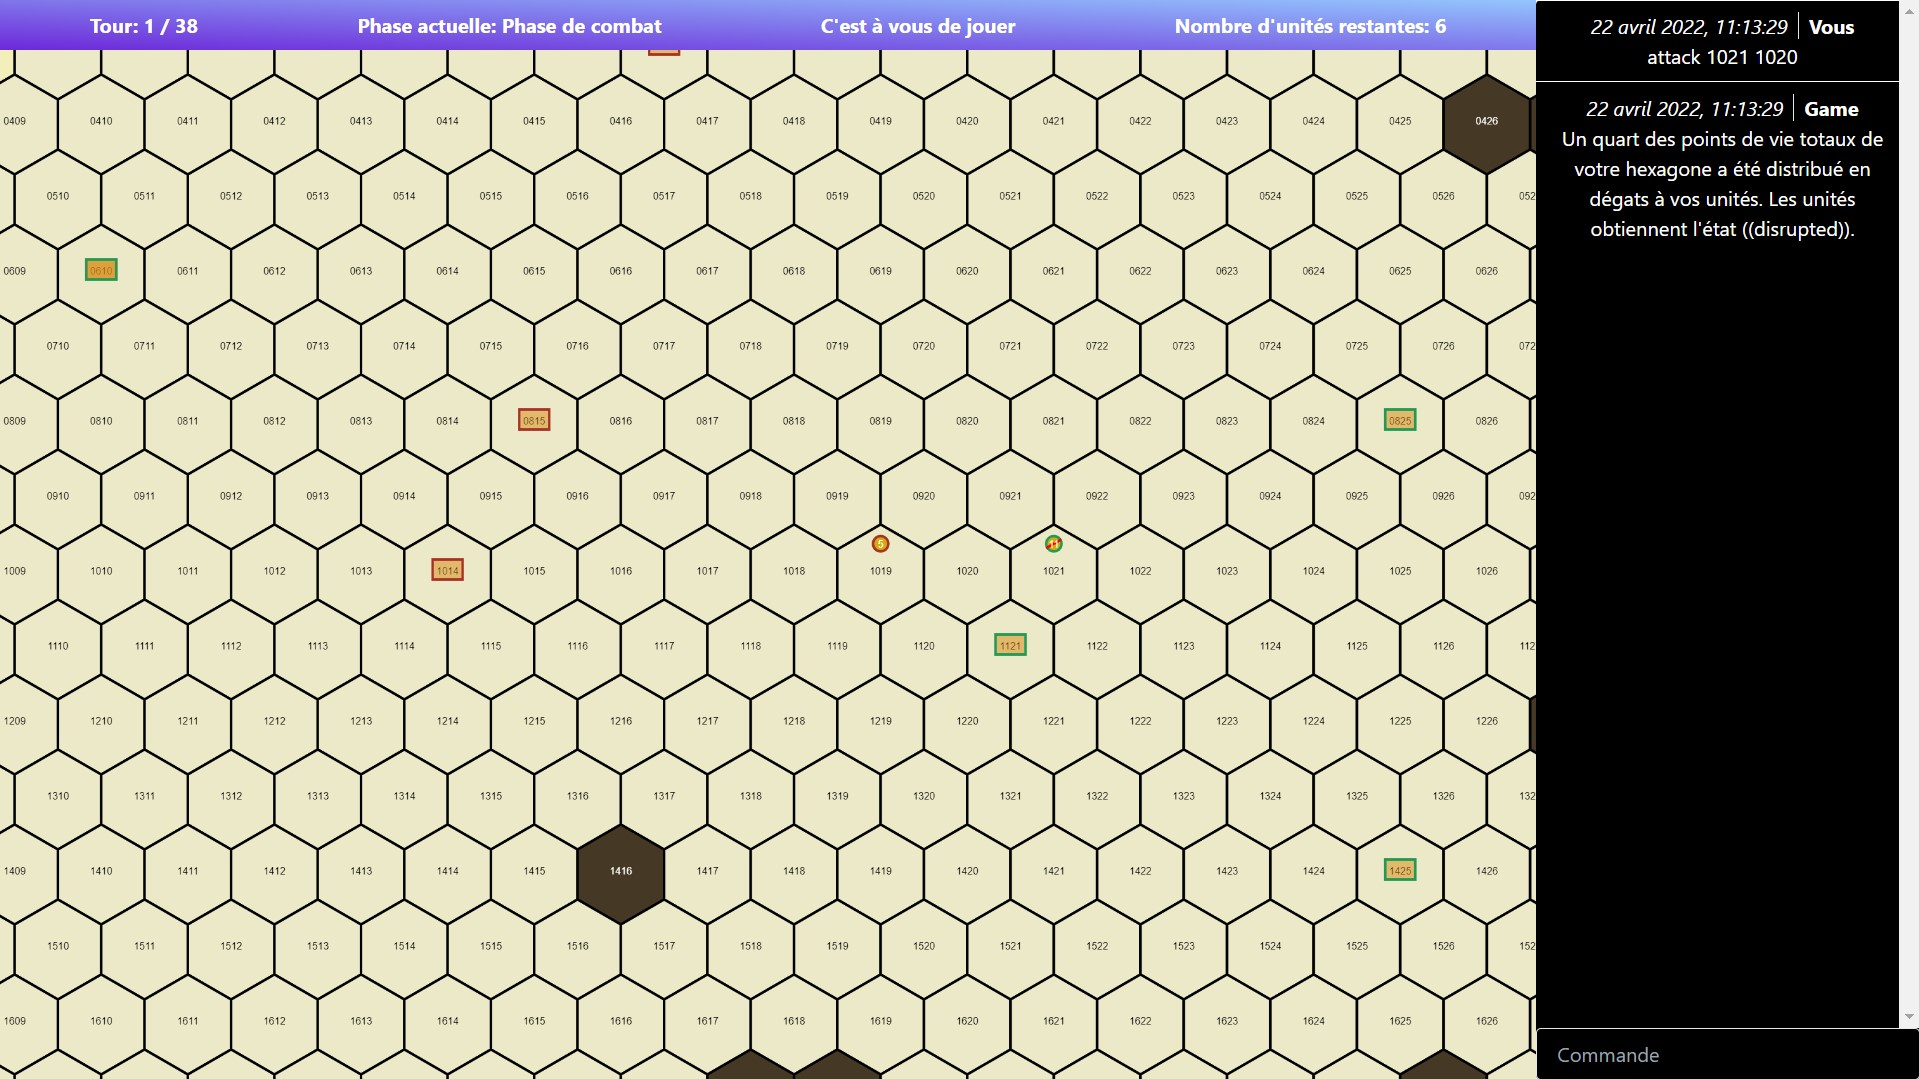
\includegraphics[scale=0.35]{data/Attacker.jpg}
    \caption{ L'exécution de la commande {\tt attack} et le résultat de cette dernière pour l'attaquant }.
\end{figure}

\begin{figure}[H]
    \centering
    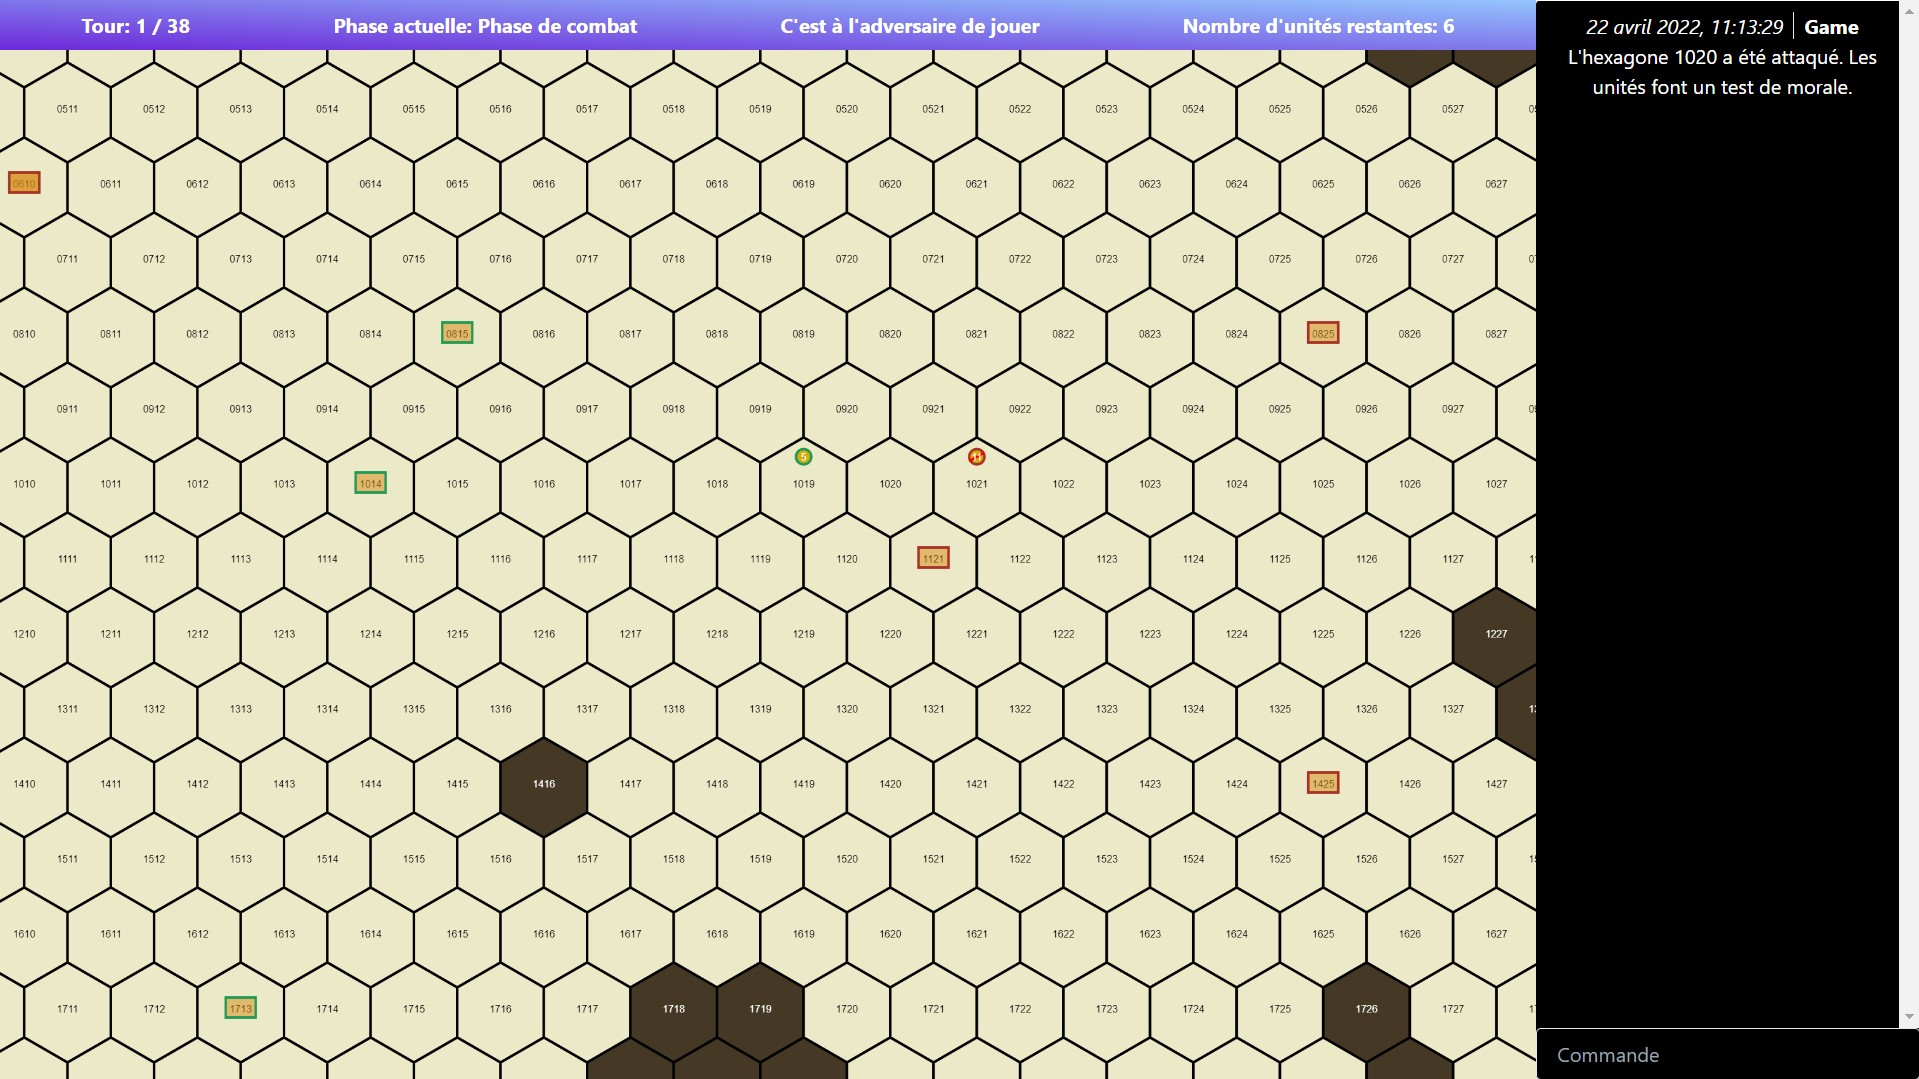
\includegraphics[scale=0.35]{data/Defender.jpg}
    \caption{L'affichage du résultat de la commande {\tt attack} pour le défendant }.
\end{figure}

Nous pouvons voir que l'attaque a échoué, et les unités attaquantes ont perdu des points de vie et sont devenues {\tt disrupted}, tandis que les unités qui défendent ont réussi à se défendre, mais font un test de morale pour vérifier si elles se replient, ce qui n'est pas arrivé dans cette situation.


Quand le joueur a terminé son tour, il doit écrire dans le terminal \og done \fg{}. Le joueur ne pourra que communiquer par chat à l'adversaire et l'adversaire peuvent continuer à jouer. Voir figure \ref{fig:fin_tour}\\





Les deux joueurs peuvent communiquer ensemble  à l'aide du terminal, le joueur doit écrire au dans le terminal \og message \fg{} puis écrit son message. Voir la figure \ref{fig:message_command} pour un exemple d'utilisation. \\


Un message d'erreur s'affiche dans le terminal si le joueur effectue des mauvaises commandes.
Par exemple, le joueur oublie des arguments ou passe des mauvais arguments. Voir figure \ref{fig:wrong_command} pour un exemple d'utilisation\\

